%% UIST 2027 full paper draft. Compile on Overleaf (acmart is built in) or with TeX Live:
%%   latexmk -pdf main.tex
%% Figures come from ../../figures/uist2027 (scripts/paper_figures.py).
%% Every number must trace to a file in results/ (docs/paper_outline.md, section 3).
%% \TODO{...} marks text that waits for data (TUAR, Study 1, Study 2) or a verified citation.
%% CHECK the UIST 2027 CFP for the required template options before submission.
\documentclass[sigconf,review,anonymous]{acmart}

\usepackage{booktabs}
\usepackage{xcolor}
\graphicspath{{../../figures/uist2027/}}
\newcommand{\TODO}[1]{\textcolor{red}{[TODO: #1]}}
\newcommand{\sqiv}{SQI\,v2}

\setcopyright{none}
\acmConference[UIST '27]{The 40th Annual ACM Symposium on User Interface Software and Technology}{October 2027}{Vienna, Austria}

\begin{document}

\title{Know When to Measure Again: Actionable Abstention for Non-Expert EEG Triage}

\author{Anonymous Author(s)}
\affiliation{\institution{Anonymous Institution}\country{}}

\begin{abstract}
Pre-hospital EEG could help route suspected stroke patients, but in the largest prehospital study a third of recordings taken by ambulance staff were not usable, and models trained on clinical EEG are easily fooled by acquisition differences.
We present a triage interface built around two ideas: tell a non-expert operator \emph{which electrode} to fix and \emph{how}, and let the system \emph{withhold} a decision with a guarantee the clinician can rely on.
The system scores every channel of a consumer headband in real time, attaches a reason and an action to each problem, and replaces ad-hoc confidence bands with patient-level conformal prediction, so that ``No-Decision'' carries a false-alert bound.
On held-out recording sources, our rule kept the realised false-alert rate at or below the target (7.7\% at $\alpha{=}0.1$), whereas the deployed fixed thresholds reached 30\% and a naive window-level calibration up to 52\%.
On 113 held-out patients with labelled artifacts, a quality score learned from the labels detected artifacts better than the deployed index but withheld half of the stroke windows, so the panel uses hand-set rules that do not penalise slowing.
\TODO{One sentence each on the two user studies, once run.}
\end{abstract}

\begin{CCSXML}
\TODO{Generate CCS concepts in the ACM tool.}
\end{CCSXML}

\keywords{EEG, signal quality, selective prediction, conformal prediction, abstention, clinical decision support, wearable sensing}

\begin{teaserfigure}
  \centering
  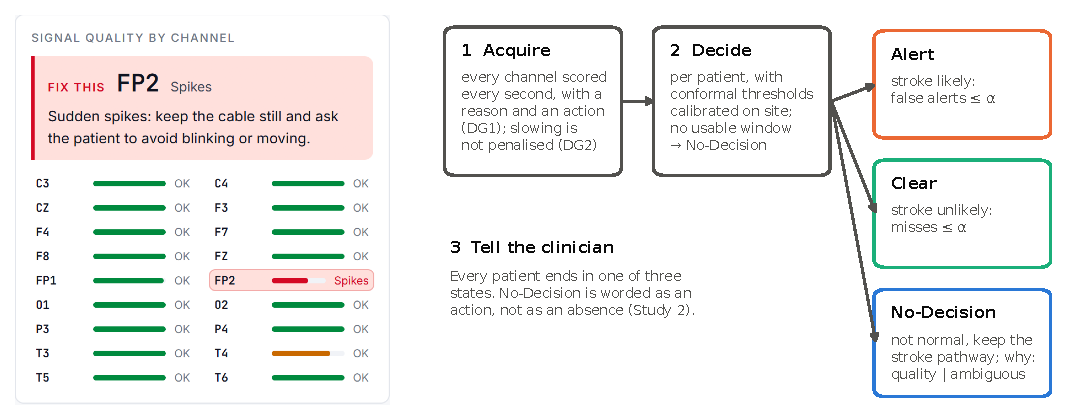
\includegraphics[width=\textwidth]{fig_teaser.pdf}
  \caption{Left: the per-channel quality panel (condition G) during the replay of an 18-channel clinical recording through the live pipeline. FP2 shows spikes that occur naturally in the recording (nothing injected); the panel names the channel, the reason and one action, while the other channels stay usable. Right: how a decision travels. Every patient ends in Alert, Clear or No-Decision, and No-Decision states why and what to do next.}
  \Description{A screenshot of a panel listing 18 EEG channels with green score bars, except FP2 which is red and labelled Spikes; a callout above reads: Fix this, FP2, Spikes, sudden spikes: keep the cable still and ask the patient to avoid blinking or moving. To the right, a flow diagram: Acquire, then Decide, then three outcome boxes labelled Alert, Clear and No-Decision.}
  \label{fig:teaser}
\end{teaserfigure}

\maketitle

%% ===================================================================================
\section{Introduction}

Acute ischemic stroke is time-critical, and an EEG taken in the ambulance could tell paramedics which patients need a thrombectomy-capable centre.
The first large prospective test of this idea, ELECTRA-STROKE, put a dry-electrode 8-channel EEG in the hands of ambulance personnel: only 212 of 311 recordings (68\%) had sufficient quality for analysis, and the authors concluded that EEG data quality needs to improve before prehospital use~\cite{vanstigt2023electra}.
The bottleneck is not only the classifier. It is whether a non-expert gets a usable signal, and what the system says when it does not.

We learned the same lesson the hard way. Our first stroke classifier reached a patient-level AUC of 0.99, yet five signal-quality features that carry no pathological information separated the classes almost as well (AUC 0.999): the stroke and control recordings came from different devices, and the model had learned the device.
When we removed the shortcuts one at a time---different sources, matched age, matched eye state---the entropy-feature model fell to an AUC of 0.57--0.73 (Section~\ref{sec:lessons}).
A system that reports such a number with confidence is dangerous; a system that refuses to report anything is useless.
Between the two lies the design space of this paper: a triage interface that helps the operator produce a usable signal and withholds a decision only when it should, with a cost that is stated in advance.

Abstention is not neutral. In a study with 259 clinicians, selective prediction reduced the harm of wrong AI advice overall but increased false negatives when the AI abstained~\cite{jabbour2025}; how the deferral is communicated changes human accuracy~\cite{bondi2022}; and a quality gate that rejects images in a deployed clinical system created friction and delays in the field~\cite{beede2020}.
An EEG triage interface therefore has to answer three questions at once: \emph{is the signal usable}, \emph{if not, what should the operator do}, and \emph{when the model abstains, what does that commit to}.

We contribute:
\begin{itemize}
  \item \textbf{A real-time, device-agnostic triage system} that scores each EEG channel with a reason code and an operator action, and runs on a 2-channel consumer headband, an 8-channel research amplifier, or replayed clinical recordings (Section~\ref{sec:system}).
  \item \textbf{Actionable abstention}: patient-level class-conditional conformal prediction that turns No-Decision into a stated false-alert bound, with the abstention reason (ambiguous evidence vs.\ poor signal) shown to the user (Section~\ref{sec:conformal}).
  \item \textbf{A technical evaluation} on held-out recording sources showing that the bound holds where fixed thresholds and window-level calibration fail, how many patients on-site calibration needs, how long a recording must be, how well the per-channel reasons and target channel match labelled artifacts, and why learning the quality score from those labels would gate stroke patients (Section~\ref{sec:techeval}).
  \item \textbf{Two user studies}: novice operators acquiring EEG with per-channel reasons and actions vs.\ a per-channel indicator only (Study~1), and clinicians deciding on vignettes under two wordings of No-Decision (Study~2) \TODO{one-line finding of each}.
\end{itemize}

%% ===================================================================================
\section{Related Work}

\paragraph{Prehospital and low-channel EEG for stroke.}
ELECTRA-STROKE showed that ambulance staff can record a dry-electrode EEG and that spectral and symmetry features carry information about large-vessel occlusion, but also that a third of recordings were unusable~\cite{vanstigt2023electra}.
Classifiers on hospital EEG report high accuracy~\cite{tong2025}, typically on cohorts where stroke and control recordings differ in acquisition; we show how much of such accuracy can be acquisition rather than pathology.
Riemannian tangent-space classifiers~\cite{barachant2012} are a strong, fast baseline for few-channel EEG and transfer better across our sources than hand-crafted entropy features.

\paragraph{Signal quality for wearable EEG.}
Quality indices for single-channel wearable EEG combine amplitude, spectral and artifact-specific features~\cite{grosselin2019}; the aperiodic spectral slope flags artifacts in single-channel recordings~\cite{fasol2023}; and the TUH Artifact Corpus provides channel-level artifact labels from one clinical system~\cite{hamid2020tuar,obeid2016tuh}.
Contact quality can also be monitored online from mains interference on a wearable EEG device, although the authors note that no accurate and reliable tool for monitoring contact during recording was yet available~\cite{casadei2022}.
These works score quality. We use per-channel quality as an \emph{interaction}: a reason, an action, and a target electrode, evaluated by whether novices acquire usable signal faster.

\paragraph{Guiding non-experts to acquire clinical signals.}
The closest precedents come from ultrasound. Real-time prescriptive guidance let nurses without ultrasonography experience acquire echocardiograms of diagnostic quality for limited questions~\cite{narang2021}, and the same approach has been applied to guide novices performing trauma ultrasound~\cite{chiu2023}.
These systems guide the probe towards a target image; EEG has no target image, so our guidance instead names the failing electrode and the physical cause (contact, drift, muscle, mains) and asks for one corrective action. We are not aware of a user study comparing such actionable feedback with the per-electrode contact indicators that EEG devices typically show; Study~1 makes that comparison.

\paragraph{Selective prediction and conformal guarantees.}
Conformal prediction gives distribution-free, finite-sample coverage~\cite{angelopoulos2021gentle}, and conformal risk control extends it to bounded losses~\cite{angelopoulos2022crc}.
On EEG, standard conformal coverage breaks when data shift across patients and personalised calibration recovers it~\cite{chatterjee2026}.
Benchmarks of EEG foundation models show that dataset identity is often decodable and must be controlled~\cite{zare2026}.
We use the simplest guarantee that matches the clinical unit---one decision per patient---and report what it costs in abstentions.

\paragraph{Clinicians and abstaining AI.}
Clinicians ignore, trust or negotiate with AI recommendations depending on how they fit the workflow~\cite{sivaraman2023}; human--AI interaction models have been translated into clinical prototypes~\cite{hussain2024}.
Selective prediction can raise false negatives when the abstention is read as reassurance~\cite{jabbour2025}, and showing a deferral without the model's prediction can improve human accuracy~\cite{bondi2022}.
Study~2 tests whether an actionable framing of No-Decision avoids the under-triage effect.

%% ===================================================================================
\section{Lessons from a Shortcut}
\label{sec:lessons}

\paragraph{Data.}
We pooled two public stroke cohorts and two public healthy-control cohorts, all openly licensed.
\emph{Xuanwu}~\cite{dataset_xuanwu}: 50 patients with acute ischemic stroke (1--30 days after onset, aged 30--77), recorded during a hand motor-imagery task.
\emph{Tianjin}~\cite{dataset_tianjin}: 24 patients with \emph{chronic} stroke (15 ischemic, 9 hemorrhagic; the per-patient type is not published), Neuracle 64-channel system; we used the rest segments of the first pre-intervention run.
\emph{Oslo}~\cite{dataset_oslo}: healthy adults, BioSemi 64-channel system, four minutes of eyes-closed rest.
\emph{PhysioNet}~\cite{dataset_eegmmidb,schalk2004,goldberger2000}: healthy adults, BCI2000 64-channel system, the one-minute eyes-open and eyes-closed baselines.
Every recording was resampled to 256\,Hz, reduced to a common 18-channel 10--20 montage, and evaluated at the patient level.
The cohorts therefore differ in device, task, eye state and stroke phase as well as in diagnosis; the rest of this section measures how much of the apparent signal each of those differences carries.

\paragraph{The confound.}
With patient-level cross-validation on 50 stroke and 50 control recordings, entropy features alone reached an AUC of 0.904. Five signal-quality features alone---flatline, clipping, line-noise and high-frequency ratios---reached 0.999, and every stroke recording came from a different device than every control.
On a single clinical system (TUH Slowing Corpus, 29 patients, slowing vs.\ background), the same quality features fell to 0.771 while entropy features reached 0.823~\cite{obeid2016tuh}: the quality shortcut is a property of the pooled cohort, not of EEG.

\paragraph{The cascade.}
Figure~\ref{fig:cascade} removes one shortcut at a time.
Within a source both models look perfect (AUC 0.993 and 0.999).
Testing on unseen sources keeps them high (0.90--0.997); matching age changes little (0.89--0.99).
Matching eye state---stroke recordings were eyes-open, one control source eyes-closed---is decisive: with eyes-open controls the feature model falls to 0.57 [0.46, 0.68] and 0.73 [0.60, 0.84], the Riemannian model holds at 0.82 [0.71, 0.90] and 0.82 [0.72, 0.90].

\begin{figure}[t]
  \centering
  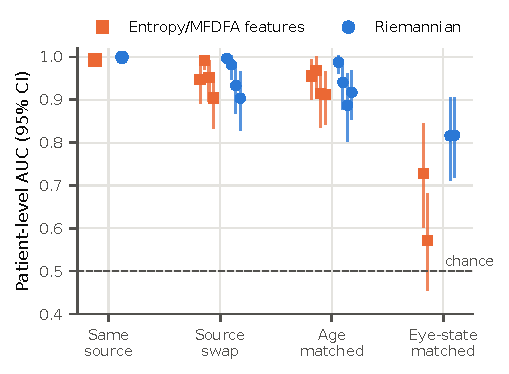
\includegraphics[width=\linewidth]{fig_confound_cascade.pdf}
  \caption{Patient-level AUC (95\% patient-bootstrap CI) as acquisition shortcuts are removed. Each point is one train/test source split. Once controls are also eyes-open, the entropy/MFDFA feature model falls to near chance while the Riemannian model keeps $\approx$0.82.}
  \Description{A dot plot of patient-level AUC with confidence intervals for two models across four control levels: within source, source swap, age matched and eye-state matched. The feature model drops from near 1.0 to between 0.57 and 0.73 at the eye-state matched level, while the Riemannian model stays around 0.82.}
  \label{fig:cascade}
\end{figure}

\paragraph{Design goals.}
The cascade turned a classification problem into an interaction problem. We derived four goals:
\textbf{DG1} --- tell the operator which electrode is the problem and what to do, not only that quality is low;
\textbf{DG2} --- never treat pathology as artifact (stroke slows and steepens the EEG spectrum, as does poor contact);
\textbf{DG3} --- when the system withholds, state what that withholding guarantees;
\textbf{DG4} --- make ``not yet known'' unmistakably different from ``normal''.

%% ===================================================================================
\section{System}
\label{sec:system}

\paragraph{Architecture.}
A FastAPI backend receives EEG over a WebSocket from a Bluetooth LE headband (2 frontal channels, 256\,Hz), an 8-channel research amplifier, or a replayed clinical recording, and feeds every chunk (0.5\,s) through the same path: per-channel quality, a causal detector with a signal-quality gate, a Riemannian tangent-space window model~\cite{barachant2012}, exponential smoothing and hysteresis, and the patient-level decision rule of Section~\ref{sec:conformal}. A browser front end renders the stream, the per-channel panel and the decision.
On a laptop CPU the Riemannian detector takes 7\,ms per 0.5\,s chunk (p95 10\,ms) and the end-to-end 18-channel path 65\,ms at p95, 13\% of real time; per-channel quality for the 2-channel headband takes 6\,ms once per second.

\subsection{Per-channel quality with reasons (\sqiv)}
\label{sec:sqi}
Every second, \sqiv{} scores the last 4\,s of each raw device channel. All features are ratios, shape statistics or log--log slopes, so the score does not depend on the recording unit:
\begin{itemize}
  \item \emph{flat} (channel 40\,dB below the median channel), \emph{missing} samples, \emph{clipping} (share of samples at the rails);
  \item \emph{line noise}: power within $\pm1$\,Hz of the mains frequency relative to 1--35\,Hz, counted only if it forms a narrow peak;
  \item \emph{muscle}: 35--70\,Hz power relative to 1--35\,Hz (mains removed), or a whitened spectrum (aperiodic exponent below 0.6);
  \item \emph{transient}: excess kurtosis;
  \item \emph{drift}: the variance below 0.5\,Hz relative to what the channel's own aperiodic $1/f$ fit predicts there,
  $\Delta_{\text{drift}} = \log_{10}\!\big(P_{<0.5\,\text{Hz}} / \int_{1/T}^{0.5} 10^{b} f^{-\chi}\,df\big)$,
  where $\chi$ and $b$ are fitted on 2--40\,Hz with the alpha and mains bands excluded.
\end{itemize}
Each feature maps to a 0--1 severity through a ramp; the channel score is one minus the weighted severities, and a reason is shown once its severity passes the ramp midpoint.
The drift definition implements DG2: a steeper $1/f$ slope or more 1--4\,Hz delta (stroke-like slowing) is predicted by the fit and is not penalised, whereas a raw ``power below 0.5\,Hz'' share grows with the exponent and gated slowed EEG as bad contact in an earlier version.
Missing alpha is reported but never penalised.
The drift ramp is fitted on half of the TUAR patients~\cite{hamid2020tuar} and frozen before evaluation: it starts at the 95th percentile of $\Delta_{\text{drift}}$ over their clean channel-windows (2.19) and saturates at 2.99.

\paragraph{Guidance (DG1).}
The panel shows every channel's score bar and, for the worst channel, a callout with the channel name, the reason and one action (e.g., ``AF3 --- slow baseline drift: press the electrode firmly or re-wet it''). Figure~\ref{fig:teaser} shows the panel during an artifact.

\subsection{Actionable abstention}
\label{sec:conformal}
Let $p$ be a patient's mean window probability of stroke over the scored windows.
We calibrate on $n_0$ control and $n_1$ stroke patients from the deployment site and set
$q_0 = \hat{Q}_{\lceil (n_0+1)(1-\alpha)\rceil}\{p_i : y_i{=}0\}$ and
$q_1 = \hat{Q}_{\lceil (n_1+1)(1-\alpha)\rceil}\{1-p_i : y_i{=}1\}$,
the finite-sample conformal quantiles of each class~\cite{angelopoulos2021gentle}.
A new patient's prediction set contains \emph{control} if $p \le q_0$ and \emph{stroke} if $1-p \le q_1$. The interface shows
\textbf{Alert} when the set is \{stroke\},
\textbf{Clear} when it is \{control\},
and \textbf{No-Decision} otherwise, with the reason \emph{ambiguous} (both classes plausible), \emph{conflict} (neither) or \emph{quality} (too few usable windows).
For exchangeable patients, $P(\text{Alert}\mid\text{control}) \le \alpha$ and $P(\text{Clear}\mid\text{stroke}) \le \alpha$ (DG3).
Two consequences follow directly and shape the interface.
First, below $\lceil 1/\alpha\rceil - 1$ calibration patients of a class, $q$ is infinite: at $\alpha{=}0.1$ the system cannot alert until 9 controls are calibrated, and it says so.
Second, the guarantee is per patient, so the streaming interface decides on the session aggregate, not on any single window (Section~\ref{sec:techeval}).

\paragraph{Framing No-Decision (DG4).}
No-Decision is shown as ``Not yet determined --- this does not mean normal'', with the reason and the next action (continue the standard stroke pathway; re-measure after fixing the named electrode), and without a probability~\cite{bondi2022}. Study~2 compares this framing with a plain one.

%% ===================================================================================
\section{Technical Evaluation}
\label{sec:techeval}

\paragraph{Setting.}
Unless stated otherwise we use the deployed Riemannian model trained on two sources and evaluated on two unseen, eye-state-matched sources: S1 (24 stroke, 50 control) and S2 (50 stroke, 50 control). On-site calibration is simulated by 2000 random stratified halves of the test patients.

\subsection{The false-alert bound holds}
Figure~\ref{fig:far} compares the realised false-alert rate with the target.
Patient-level conformal stays at or below $\alpha$ in both splits (S1: 0.039, 0.077, 0.191 at $\alpha = 0.05, 0.1, 0.2$; S2: 0.039, 0.076, 0.186).
The fixed thresholds of the deployed detector (alert at $p \ge 0.8$) give 0.30 in S1 and 0.16 in S2, independent of any target.
Calibrating on windows and alerting when any window crosses the threshold---what a naive streaming implementation does---gives 0.11--0.52, two to five times the target, because windows of one patient are correlated.
The cost is abstention: at $\alpha = 0.1$, 64\% (S1) and 71\% (S2) of stroke patients fall into No-Decision; at $\alpha = 0.2$, 29\% and 15\%, with sensitivity 0.57 and 0.67. Almost no stroke patient is cleared (miss $\le \alpha$), which is why the framing of No-Decision matters (Study~2).
The bound also holds behind the quality gate the interface uses. Scoring each window on the raw signal with \sqiv{} (frozen ramp) and dropping windows below the channel threshold removed 16\% of control and 1\% of stroke windows; seven of 50 controls had no usable window and always received No-Decision with reason ``quality''. The realised false-alert rate stayed at or below $\alpha$ in both splits (S1: 0.039, 0.079, 0.155; S2: 0.039, 0.077, 0.151).

\begin{figure*}[t]
  \centering
  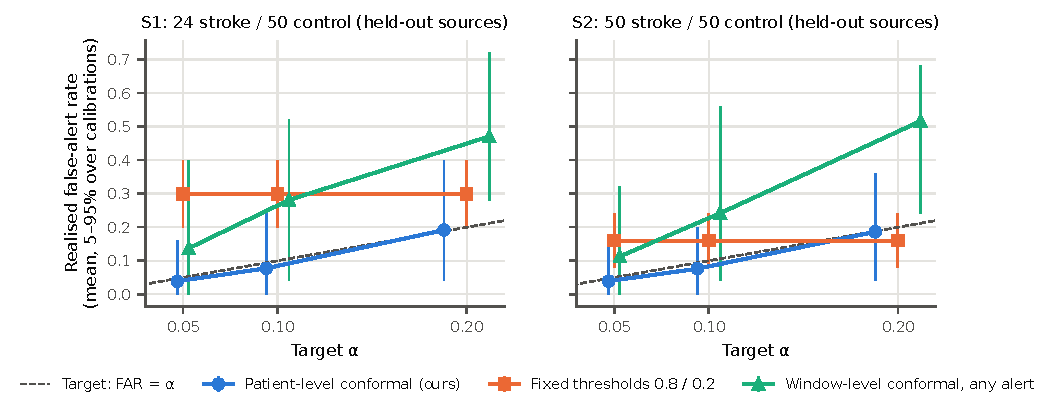
\includegraphics[width=0.85\linewidth]{fig_far_vs_alpha.pdf}
  \caption{Realised false-alert rate (mean, 5--95\% over 2000 calibration draws) against the target $\alpha$ on two held-out source splits. Only patient-level conformal tracks the dashed target; fixed thresholds ignore it and window-level calibration with ``any alert'' exceeds it severalfold.}
  \Description{Two line charts, one per held-out split, plotting the realised false-alert rate against the target alpha from 0.05 to 0.2. The patient-level conformal line follows the dashed identity line; the fixed-threshold line is flat at 0.30 or 0.16; the window-level line lies two to five times above the target.}
  \label{fig:far}
\end{figure*}

\subsection{How many calibration patients?}
The bound is marginal over calibration draws. Figure~\ref{fig:calsize} shows that with 9--20 calibration patients per class the mean false-alert rate stays at or below 0.1, following the theoretical sawtooth $1-\lceil (n+1)(1-\alpha)\rceil/(n+1)$, but a single site's realised rate varies: in 9--21\% of draws it exceeds $\alpha + 0.05$, and its 90th percentile reaches 0.22. A site that wants a per-site guarantee needs more calibration patients or a calibration-conditional bound; we expose this in the interface as the number of calibration patients behind the current $\alpha$.

\begin{figure}[t]
  \centering
  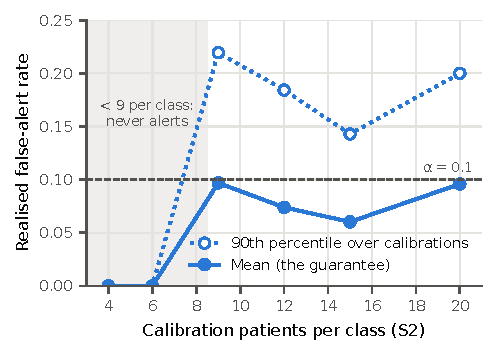
\includegraphics[width=\linewidth]{fig_calibration_size.pdf}
  \caption{False-alert rate at $\alpha = 0.1$ against the number of calibration patients per class (S2, 1000 draws). Below 9 per class the system can never alert. The mean respects $\alpha$; the 90th percentile shows what a single site may experience.}
  \Description{A line chart of false-alert rate against the number of calibration patients per class. The mean follows a sawtooth at or below 0.1 from 9 patients onward and is zero below 9; the 90th percentile line lies higher, up to about 0.22.}
  \label{fig:calsize}
\end{figure}

\subsection{How long to record?}
Streaming each S2 recording through the deployed detector and scoring patients from the first $T$ seconds (Figure~\ref{fig:time}), the patient AUC is 0.79 after 8\,s and 0.80 after 120\,s; the false-alert rate stays at 0.08 for $\alpha = 0.1$ at every horizon. Recording longer does not make the model more accurate, so the time that matters is the time to a usable signal, which Study~1 measures. The flat curve also indicates that the model reads stationary properties of a recording, which may still include source traits.

\begin{figure}[t]
  \centering
  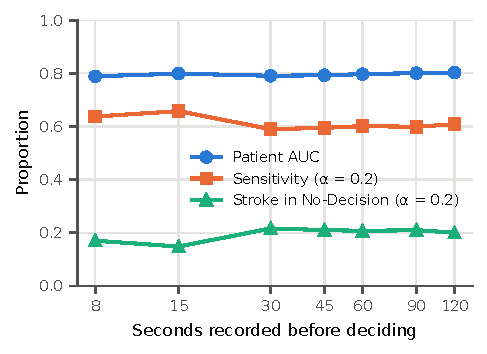
\includegraphics[width=\linewidth]{fig_decision_time.pdf}
  \caption{Patient AUC, sensitivity and share of stroke patients in No-Decision ($\alpha = 0.2$) against the seconds recorded before deciding (S2, 50 stroke / 50 control).}
  \Description{A line chart against seconds recorded, from 8 to 120 seconds: patient AUC stays between 0.79 and 0.80, sensitivity between 0.59 and 0.66, and the share of stroke patients in No-Decision between 0.15 and 0.22.}
  \label{fig:time}
\end{figure}

\subsection{Per-channel quality on labelled artifacts}
We use the TUH artifact corpus (TUAR v3.0.1~\cite{hamid2020tuar}): 310 clinical recordings of 213 patients with artifacts annotated per bipolar channel. A 4\,s channel-window counts as an artifact when an annotation covers at least half of it and as clean when none touches it. Patients are split by a salted hash into a calibration half (100), used only to fix the drift ramp, and a test half (113 patients, 157 recordings, 532k channel-windows, 38\% artifact). All intervals resample patients (2000 draws).

\paragraph{Detection.}
The hand-set \sqiv{} rule detects labelled artifacts \emph{worse} than the deployed index: AUC 0.708 vs.\ 0.743 (difference $-0.035$ [$-0.063$, $-0.008$]). The \sqiv{} features nevertheless carry more information: a logistic model over them, cross-fitted by patient, reaches 0.827 vs.\ 0.746 over the deployed index's features ($+0.081$ [0.048, 0.117]), which passes our pre-registered rule (gain $\ge 0.05$) on the point estimate but not on the lower bound. The gain comes from eye movements ($+0.18$) and electrode artifacts ($+0.21$); muscle and chewing are detected equally well by both.

\paragraph{A learned score breaks DG2.}
We therefore fitted that model on the calibration half and froze it with a threshold that flags 5\% of clean channel-windows (plan committed before fitting). On the test half it beat the deployed index by $+0.081$ [0.057, 0.109]. On our stroke cohorts, however, it withheld 51\% of stroke windows and 0.3\% of control windows, and its mean score alone separated the two (AUC 0.006, i.e., near-perfect in reverse): its largest weight is on the aperiodic exponent, which stroke slowing and device differences both shift. The one variant we had fixed in advance, without the delta and alpha features, failed the same way (45\% vs.\ 0.1\%). We kept the hand-set rule. A quality score learned from artifact labels on one clinical system becomes a detector of the recording source or of the pathology itself; for a triage system this is the worst failure, because it withholds decisions from exactly the patients it is for.

\paragraph{Reasons and target channel.}
\sqiv{} gives a reason for 50\% of artifact channel-windows; when it does, the reason matches the labelled type in 71\%. Most eye movements (86\%) get no reason, and 22\% of muscle windows are called drift. The channel the interface points at carries the labelled artifact in 53\% of windows with both artifact and clean channels, against 38\% by chance and 54\% for the deployed index (difference [$-0.044$, 0.039]). We tried to close the eye-movement gap with an advisory reason that cannot change any score (high 1--4\,Hz share without alpha; thresholds fixed on the calibration half, criteria fixed beforehand). On the test half it raised correct reasons for eye movements from 6\% to 31\% while firing on 3.8\% of clean channels, but it lowered overall reason accuracy to 68\% and fired five times as often on stroke as on control channels (7.5\% vs.\ 1.5\%). Per channel, eye movements and stroke slowing look alike, so we did not ship it. The per-channel reasons are thus a useful but imperfect description; we do not claim that \sqiv{} localises artifacts better than a per-channel version of the deployed index, and Study~1 tests whether the reasons and actions help operators.

\paragraph{Slowing is not gated as artifact (DG2).}
With the frozen drift ramp, \sqiv{} withheld fewer slowing segments than background segments on one clinical system (TUSL, 30.5\% vs.\ 47.5\% of windows) and fewer stroke than control windows across sources (0.3\% of 50 stroke vs.\ 15.7\% of 50 control recordings, the latter mostly mains interference on the 60\,Hz control rig). Its record score separates the stroke and control sources with AUC 0.61, against 0.999 for the deployed index's features (Section~\ref{sec:lessons}), so the hand-set rule carries far less of the acquisition shortcut.

\paragraph{A real headband recording.}
On a 19\,s recording from the 2-channel headband whose first seconds were dominated by slow drift (90--98\% of variance below 0.5\,Hz), the deployed quality index passed all 37 windows (mean 0.95). With the frozen ramp, \sqiv{} asked the operator to press or re-wet AF3 once, in the window ending at 9\,s ($\Delta_{\text{drift}} = 2.76$), and flagged three windows with transients. The first 10\,s had $\Delta_{\text{drift}}$ between 1.6 and 2.8, at the onset of the ramp: a threshold set at the 95th percentile of clean clinical channels is lenient for a dry headband, and a device-specific ramp would have flagged the whole drift episode, as the synthetic default did.

%% ===================================================================================
\section{Study 1: Novice Acquisition}
\label{sec:study1}
Study~1 asks whether telling a novice \emph{why} a channel is poor and \emph{what to do} gets usable EEG faster than telling them only \emph{which} channel is poor.
The analysis plan below is fixed before the first session \TODO{pre-register on OSF and link (anonymised) here}.

\paragraph{Participants.}
Sixteen operators who had never placed EEG electrodes (\TODO{demographics; how many were paramedics or nurses}) and four healthy wearers, all adults; each wearer was recorded by several operators.
Sixteen operators give 80\% power for a paired effect of $d=0.8$ at $\alpha=0.05$ and fill both counterbalancing orders; two to three pilot operators, not counted, check the effect-size assumption \TODO{pilot outcome}.

\paragraph{Conditions.}
Both conditions used the same application, headband (2-channel, AF3/AF4, Bluetooth) and live trace.
In \textbf{B}, every channel showed a quality bar and an OK/Poor label, the indicator found in clinical impedance checks and consumer headbands.
In \textbf{G}, the same bars were joined by the \sqiv{} reason, one corrective action and the channel to fix first (Section~\ref{sec:sqi}).
The only difference between conditions is therefore the reason and the action, which is the contribution under test.
Operators were not told which condition was new.

\paragraph{Task and faults.}
Each trial started with three scripted faults drawn from four: a dry electrode, a loose band, a jaw clench held until the operator asked the wearer to relax, and a powered charger beside the device (mains noise).
Both conditions used the same fault set in a different order.
The instruction was ``obtain 60 seconds of good signal as fast as you can'' with an 8-minute limit, thinking aloud.
Each operator did one trial per condition with a different wearer; condition order, wearer and fault set were balanced with a Latin square.
After each trial operators completed NASA-TLX and SUS; a 10-minute semi-structured interview closed the session.

\paragraph{Measures.}
The primary outcome is time to usable signal (TTU): the start of the first run of 60\,s that an independent EEG reader rated usable, measured from the trial start marker.
The application stored each raw recording under an opaque identifier; the reader rated shuffled 10\,s epochs, plotted at a fixed per-recording scale, without knowing operator, condition or time.
A second reader rated 20\% of epochs (Cohen's $\kappa$).
We did not use \sqiv{} itself as the outcome, since that would favour G.
Secondary outcomes: success within 8 minutes, correct identification of the fault cause (coded from think-aloud by two coders), number of corrective actions (application log), NASA-TLX, SUS and trust~\cite{jian2000trust}.

\paragraph{Analysis.}
H1 (G shortens TTU): Wilcoxon signed-rank on paired TTU, trials without a usable run set to 8 minutes; sensitivity analysis with a Cox model with operator frailty, treating those trials as censored.
Success: McNemar. Fault identification: logistic GLMM with operator and fault-type random intercepts. Effect sizes are reported with 95\% operator-level bootstrap intervals, and order effects are checked.

\paragraph{Results.}
\TODO{TTU by condition (paired plot), success, fault identification, NASA-TLX/SUS, $\kappa$, qualitative themes.}

\section{Study 2: Framing No-Decision}
\label{sec:study2}
The conformal rule rarely clears a stroke patient; it places them in No-Decision instead.
When an AI declines to answer, clinicians can under-diagnose more than with no AI at all~\cite{jabbour2025}, so the wording of No-Decision decides whether the risk it holds becomes a missed stroke.
Study~2 compares two wordings.

\paragraph{Participants.}
Emergency and neurology physicians, emergency nurses and final-year medical students; at least 40 (20 per framing), target 60 \TODO{actual N, roles, years of experience}.

\paragraph{Materials.}
Twenty-four pre-hospital vignettes, 12 strokes and 12 mimics (hypoglycaemia, post-ictal state, migraine with aura, Bell's palsy, \ldots), each with age, sex, time of onset, vital signs, a short NIHSS-style examination and the EEG system's output screen. A neurologist validates the reference answer and difficulty of each vignette before the study \TODO{clinical advisor not yet recruited; state their role once done}.
Within subjects, every participant saw four output types: no AI (6 vignettes), alert (4; one wrong), clear (4; one wrong) and No-Decision (10; 5 strokes, 5 mimics). Four rotated lists paired each vignette with each output type across the sample.
Between subjects, No-Decision was worded either \textbf{plain} (``Not certain enough to give a result'') or \textbf{actionable} (``Undetermined --- this does not mean normal. The signal cannot rule out stroke. Continue the standard stroke pathway. You may re-record after adjusting electrode AF4.''), with the reason (\texttt{ambiguous} or \texttt{quality}) in words and no probability~\cite{bondi2022}.

\paragraph{Procedure and measures.}
Online, about 25 minutes. For each vignette: activate the stroke pathway and transfer to a stroke centre (yes/no), confidence (1--7) and influence of the EEG result (1--7). At the end, participants explained in their own words what No-Decision meant. Two attention checks were excluded by a pre-registered rule.

\paragraph{Analysis.}
H5 (actionable wording raises activation on stroke vignettes with No-Decision): logistic GLMM, activation $\sim$ framing + (1\,|\,participant) + (1\,|\,vignette), stroke No-Decision vignettes only, reported as an odds ratio with 95\% CI.
H6/H7: on stroke vignettes, output (no AI vs.\ No-Decision) $\times$ framing; H7 tests non-inferiority of actionable No-Decision against no AI with a 10-point margin fixed in advance.
With 40 participants the study detects only large differences ($\approx$20 points), so we report effect sizes with intervals, not only $p$-values.
The cost of the actionable wording is measured as activation on mimic vignettes with No-Decision.

\paragraph{Results.}
\TODO{Activation by framing and output type, mimic over-triage, confidence, coded meanings of No-Decision.}

%% ===================================================================================
\section{Discussion}

\paragraph{$\alpha$ is an interaction parameter.}
The same model and data give 8\% false alerts with 64--71\% of stroke patients withheld, or 19\% false alerts with 15--29\% withheld. Neither is ``the accuracy''; the choice belongs to the clinical service and should be visible in the interface together with the number of calibration patients behind it.

\paragraph{Abstention moves risk; framing decides where it lands.}
The conformal rule almost never clears a stroke patient, so the risk sits in No-Decision. Whether that risk becomes a missed stroke depends on how No-Decision is read~\cite{jabbour2025}; Study~2 measures this directly.

\paragraph{Beyond stroke.}
Nothing in the quality layer or the decision rule is specific to stroke. Per-channel guidance and patient-level abstention apply to any EEG triage task acquired by non-experts, for example reduced-montage seizure screening in the emergency department, where rapid EEG systems already pair simplified acquisition with automated detection~\cite{richard2024rapideeg}.

\paragraph{Limitations.}
Our stroke and control recordings come from different public sources; even our most controlled split cannot separate pathology from acquisition completely, and we make no diagnostic claim.
The 2-channel headband is used for quality and guidance only; classification uses 18-channel recordings.
The conformal bound assumes exchangeable patients at the deployment site and is marginal over calibration draws.
The drift threshold is calibrated on one clinical system (TUAR) and is lenient for the dry headband; the reasons miss most eye movements.
Study~1 operators were mostly novices recruited on campus, a proxy for paramedics who work under time pressure in a moving vehicle; the scripted faults are common causes of poor contact but not an exhaustive set, and healthy wearers do not move, sweat or vomit like patients.
Study~2 uses vignettes, not patients, so it measures stated decisions rather than actual transfers, and its sample detects only large framing effects.

\section{Conclusion}
\TODO{Two to three sentences once all results are in.}

\bibliographystyle{ACM-Reference-Format}
\bibliography{references}

\end{document}
